\section{Data}\label{sec:Data}

\subsection{HMDA Data}\label{subsec:HMDA_Data}

The main dataset was retrieved from the HMDA Data Browser\footnote{https://ffiec.cfpb.gov/data-browser/data/2022?category=states} (see \textbf{chapter \ref{subsec:mortgage_lending_fairness}}). 
The data selection process is loosely based on the paper by Ghoba and Colaner (\cite{Ghoba}, see \textbf{chapter \ref{subsec:mortgage_lending_fairness}}), but adjusted to the scope of this thesis (see below).
All data were generated in \textbf{2022}, which supports the claim of this thesis to provide data that are newer than the studies available and potentially already include effects from the COVID pandemic. 
\textbf{All financial institutions} were included, but to narrow down the research focus to racial fairness specifically, the approach of Ghoba and Colaner was followed by only including the two predominant racial groups (\textbf{Non-Hispanic White} and \textbf{Black or African Americans}) in the analysis. 
In terms of geographical filtering, inspiration was drawn from the paper by Singh et al. (\cite{Singh2022}, see \textbf{chapter \ref{subsec:mortgage_lending_fairness}}), but instead of including different-sized states, a fairness-based approach was taken: 
U.S.News publishes a ranking of US states by their equality, by measure of distributions by race, gender and other fairness-related aspects and aggregate them to overall equality levels\footnote{2023 ranking:https://www.usnews.com/news/best-states/rankings/opportunity/equality?sort=rank-desc, methodology: https://www.usnews.com/news/best-states/articles/methodology}. 
To use a subset of the HMDA data that is likely to include fairness issues, the five states considered least equal in the year 2023 were included in the data, being \textbf{South Dakota, Louisiana, Utah, Texas,} and \textbf{Montana}. The resulting dataframe has \textit{867.401 rows and 99 columns}.

The features included for the analysis are close to the ones proposed by Ghoba and Colaner to maintain a degree of comparability, but adjusted to the scope of this thesis by including a different target variable as well as different geographical features: 
\textit{action\_taken, county\_code, interest\_rate, applicant\_sex, applicant\_race-1, loan\_type, debt\_to\_income\_ratio, loan\_to\_value\_ratio,} and \textit{lien\_status}\footnote{https://ffiec.cfpb.gov/documentation/publications/loan-level-datasets/lar-data-fields}. 
Missing values were present in \textit{interest\_rate (320.335), loan\_to\_value\_ratio (257.408), debt\_to\_income\_ratio (229.442),} and \textit{county\_code (9.053)}. 
Furthermore, three columns contained the string \textit{Exempt} as a value \textit{(interest\_rate: 20.591 occurrences; loan\_to\_value\_ratio, and debt\_to\_income\_ratio: 20.533 occurrences each)}, preventing them from initially being cast as numerical types.
In order to clean and reshape the data in a easily analyzable format, several steps were taken that are described in the following and summarized in \textbf{table \ref{tab:HMDA_transformation_summary}}.

\begin{table}[h]
    \centering
    \begin{tabularx}{\textwidth}{l *{3}{>{\centering\arraybackslash}X}}
    \hline
     & \textbf{Transformation Step} & \textbf{Reasoning} \\
    \hline
    \textbf{Rows with missing county code} & Dropping & Insignificant amount, imputation not feasible, presumably MCAR \\
    \textbf{All variables} & Typecasting & Required for further analysis \\
    \textbf{loan\_granted} & Creation & Target variable for the classification task \\
    \textbf{Exempt} & Recoding & Recoding to zero for proper typecasting \\
    \textbf{debt\_to\_income\_ratio} & Binning & Reduction of total categories \\
    \textbf{loan\_to\_value\_ratio} & Outlier Removal & Few outliers skewed the initial distribution \\
    \textbf{interest\_rate} and \textbf{loan\_to\_value\_ratio} & Imputation & Mean Imputation to tackle missingness \\
    \hline
    \end{tabularx}
    \medskip
%    \caption{Transformation Steps in the HMDA Mortgage Data}
%    \small
%    Several transformation steps have been applied to the HMDA mortgage data in order to make it easily analyzable.
%    \caption[Explainability Overview, from \cite{SALEEM2022165}]{\textbf{Explainability Overview, from \cite{SALEEM2022165}} - The concept of \textit{explainability} must be understood in the context of similar and related concepts like \textit{understandability}.}
    \caption[Transformation Steps in the HMDA Mortgage Data]{\textbf{Transformation Steps in the HMDA Mortgage Data} - Several transformation steps have been applied to the HMDA mortgage data in order to make it easily analyzable.}
    \label{tab:HMDA_transformation_summary}
\end{table}

All rows including missing values for the \textit{county\_code} were \textbf{dropped}, as their relative amount was insignificant, imputation was not logically possible for this variable, and missingness completely at random could be assumed from visual inspection using the missingno package\footnote{https://github.com/ResidentMario/missingno} (see \textbf{Figure~\ref{fig:CH03_Missingno_Completeness}}). 
All features were \textbf{cast} to their appropriate types \textit{(county\_code: string; applicant\_race-1, applicant\_sex, lien\_status, loan\_type: category)}. Furthermore, a \textbf{new target variable} \textit{(loan\_granted)} was created from \textit{action\_taken} (which was dropped), assuming 1 for granted loans and 0 for denials instead of including different reasons for (dis-)approval.

\begin{figure}[h]
    \centering
    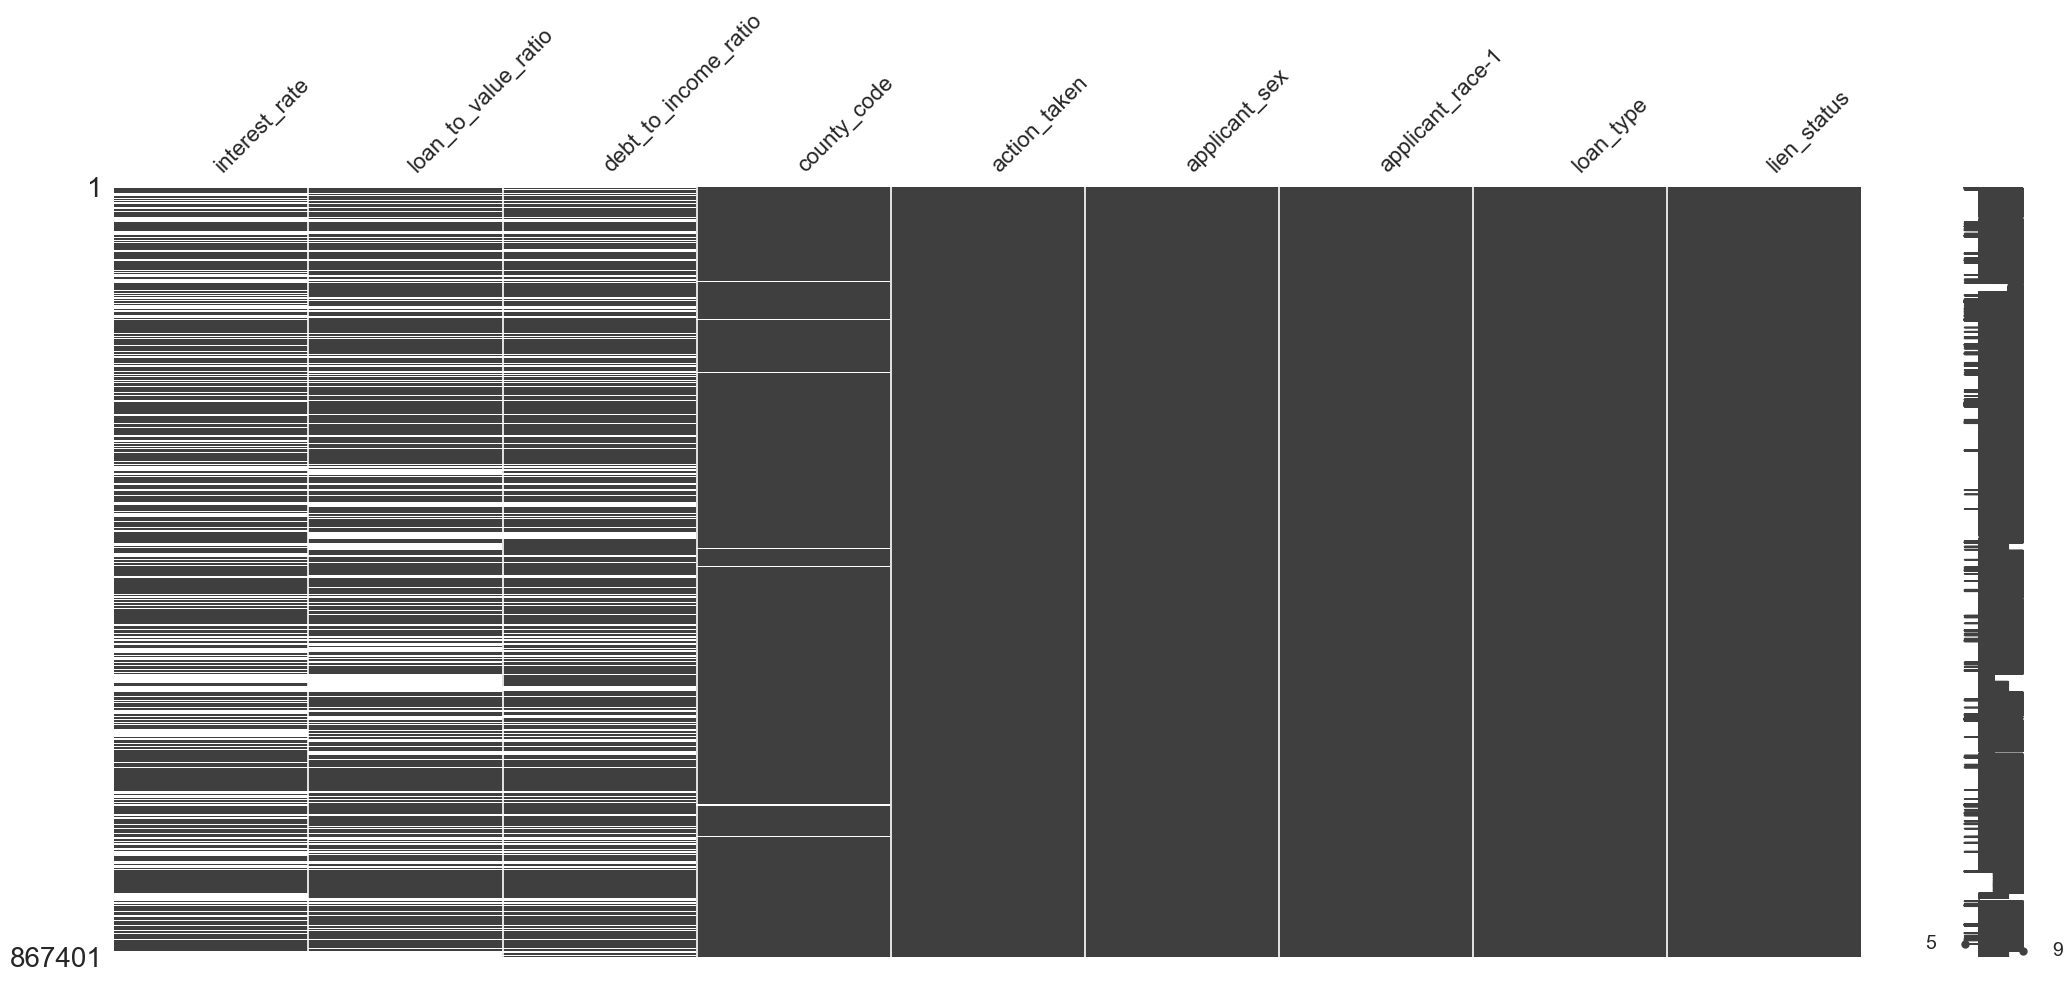
\includegraphics[width=1\textwidth]{images/CH03_Missingno_Completeness.png}
%    \caption{Visual Inspection of Missingness in the missingno Package}
%    \medskip
%    \small
%    Visual Inspection of Missingness shows that some datapoints seem to be missing at random in \textit{interest\_rate}, \textit{loan\_to\_value\_ratio}, and \textit{debt\_to\_income\_ratio}, while the other features expose no or very little missingness.
    \caption[Visual Inspection of Missingness in the missingno Package]{\textbf{Visual Inspection of Missingness in the missingno Package} - Visual Inspection of Missingness shows that some datapoints seem to be missing at random in \textit{interest\_rate}, \textit{loan\_to\_value\_ratio}, and \textit{debt\_to\_income\_ratio}, while the other features expose no or very little missingness.}
    \label{fig:CH03_Missingno_Completeness}
\end{figure}

All \textit{Exempt} strings were \textbf{recoded} as zero, allowing proper typecasting (float) for the \textit{interest\_rate} and \textit{loan\_to\_value\_ratio} variables. 
For \textit{\_to\_income\_ratio}, further \textbf{binning} was introduced, creating the new categories \textit{36\%-41\%, 41\%-45\%}, and \textit{46\%-49\%}. %Initially, Missingness was encoded as a separate category, bringing the number of distinct values for \textit{debt\_to\_income\_ratio} to eleven. 
%This was kept, because later analysis showed that missingness in the \textit{debt\_to\_income\_ratio} was a feature that heavily impacted predictions: As a comparison, a random forest classifier was trained to predict the missingness in the \textit{debt\_to\_income\_ratio} based on the other features.
%Although only a 63.7\% accuracy was achieved on the test data, the model was used to impute the missing values in the \textit{debt\_to\_income\_ratio} column, as this methodology still is more thorough than other imputation methods for categorical values like using the mode. As per the predictions, most of the missing values (125,312) were imputed as \textit{>61\%}, followed by \textit{50\%-60\%}. 
%Because later analysis proved that encoding as missingness was way more beneficial to the performance metrics, this option was finally included.
As later analysis suggested that missingness in the \textit{debt\_to\_income\_ratio} was a feature that heavily impacted predictions, the missingness was encoded as a separate category.
After assessing the distributions of \textit{interest\_rate} and \textit{loan\_to\_value\_ratio}, extreme outlier values \textit{(loan\_to\_value\_ratio > 250)} were \textbf{dropped}. 

To tackle missingness in \textit{interest\_rate} and \textit{loan\_to\_value\_ratio}, \textbf{imputation} was utilized. 
As the preferred way of imputing, the KNNImputer from the scikit-learn package\footnote{https://scikit-learn.org/stable/}, proved to be too computationally expensive to be efficiently used, the IterativeImputer from the same package was used as an alternative. 
This multivariate imputing technique is supposed to infer feature values from other features\footnote{https://scikit-learn.org/stable/modules/generated/sklearn.impute.IterativeImputer.html}. It is however set up to default to the mean as the imputation value if no satisfying solution is found.%, which was the case in the data.

In order to prepare the HMDA data for the classification task, the numerical variables \textit{(interest\_rate, loan\_to\_value\_ratio)} were \textit{standardized} using Z-score standardization: 

\begin{equation}
    z = \frac{x - \mu}{\sigma}
    \label{eq:Z-Score Standardization}
    \addcontentsline{frm}{formulas}{\protect\numberline{\theequation}\hspace{1em}Z-Score Standardization}
\end{equation}

The target variable \textit{loan\_granted} was \textbf{encoded} as a binary variable. Furthermore, all categorical variables were \textbf{one-hot encoded}, dropping the first column to avoid multicollinearity.
The data was \textbf{split} into \textit{train, test}, and \textit{validation} sets with an 80/20 split each using the \textit{train\_test\_split} function from sklearn.
These steps add to the list of transformation steps that were applied to the HMDA mortgage data, which are summarized in \textbf{table \ref{tab:HMDA_transformation_summary_2}}.

\begin{table}[h]
    \centering
    \begin{tabularx}{\textwidth}{l *{3}{>{\centering\arraybackslash}X}}
    \hline
     & \textbf{Transformation Step} & \textbf{Reasoning} \\
    \hline
    \textbf{Rows with missing county code} & Dropping & Insignificant amount, imputation not feasible, presumably MCAR \\
    \textbf{All variables} & Typecasting & Required for further analysis \\
    \textbf{loan\_granted} & Creation & Target variable for the classification task \\
    \textbf{Exempt} & Recoding & Recoding to zero for proper typecasting \\
    \textbf{debt\_to\_income\_ratio} & Binning & Reduction of total categories \\
    \textbf{loan\_to\_value\_ratio} & Outlier Removal & Few outliers skewed the initial distribution \\
    \textbf{interest\_rate} and \textbf{loan\_to\_value\_ratio} & Imputation & Mean Imputation to tackle missingness \\
    \textbf{interest\_rate} and \textbf{loan\_to\_value\_ratio} & Standardization & Z-Score Standardization for better model performance \\
    \textbf{Categorical Variables} & One-Hot Encoding & Required for model training \\
    \textbf{Data} & Splitting & Train, Test, and Validation sets for model training and testing \\
    \hline
    \end{tabularx}
%    \caption{Transformation Steps in the HMDA Mortgage Data (including preparation for model training and testing)}
%    \small
%    Several transformation steps have been applied to the HMDA mortgage data in order to make it easily analyzable.
    \medskip
    \caption[Transformation Steps in the HMDA Mortgage Data (including preparation for model training and testing)]{\textbf{Transformation Steps in the HMDA Mortgage Data (including preparation for model training and testing)} - Several transformation steps have been applied to the HMDA mortgage data in order to make it easily analyzable.}
    \label{tab:HMDA_transformation_summary_2}
\end{table}

\pagebreak

\subsection{Enrichment Data}\label{subsec:Enrichment_Data}

The enrichment data was obtained from the \textit{\href{https://www.ers.usda.gov/data-products/county-level-data-sets/}{USDA ERS page}}\footnote{https://www.ers.usda.gov/data-products/county-level-data-sets/}. All data used are structured, tabular data that are publicly available. Privacy concerns are not relevant, as the data is anonymized and aggregated. All available reports were downloaded, specifically the following datasets:

\begin{itemize}
    \item \textbf{Poverty} (2021 latest)
    \item \textbf{Population} (2022 latest)
    \item \textbf{Unemployment, and Median Household Income} (annual average 2022 unemployment and 2021 median income latest)
    \item \textbf{Education} (2017–21, 5-year average latest).
\end{itemize}

In order to clean and reshape the data in a easily analyzable format, several steps were taken that are described in the following and summarized in \textbf{table \ref{tab:enrichment_transformation_summary}}. %\footnote{For all detail, see the corresponding cleaning notebook at !!! XXX !!!}:

\begin{table}[h]
    \centering
    \begin{tabularx}{\textwidth}{l *{3}{>{\centering\arraybackslash}X}}
    \hline
     & \textbf{Transformation Step} & \textbf{Reasoning} \\
    \hline
    \textbf{Geography} & Filtering & Only include the five states in question \textit{("SD", "LA", "UT", "TX", "MT")} \\
    \textbf{Year} (where applicable) & Filtering & Only include the newest datapoints \\
    \textbf{Features} & Reducing & Only include the most relevant features \textit{(Poverty, Population, Unemployment and Median Household Income, Education)} \\
    \textbf{Data Structure} & Pivoting & Use the attributes as feature names \\
    \textbf{Indexing} & Indexing & Use the FIPS code and the name of the respective county as index \\
    \textbf{Renaming} & Renaming & Rename the feature columns for clarity \\
    \textbf{Merging} & Merging & Merge all datasets into a single dataframe \\
    \hline
    \end{tabularx}
%    \caption{Transformation Steps in the Enrichment Data}
%    \small
%    Several transformation steps have been applied to the geographical enrichment data in order to make it easily analyzable.
    \medskip
    \caption[Transformation Steps in the Enrichment Data]{\textbf{Transformation Steps in the Enrichment Data} - Several transformation steps have been applied to the geographical enrichment data in order to make it easily analyzable.}
    \label{tab:enrichment_transformation_summary}
\end{table}

All datasets were \textit{filtered} to only contain county-level data for the five states in question \textit{("SD", "LA", "UT", "TX", "MT")}, not the aggregated values for the full states, and, in case multiple years of analysis were available, to only include the newest datapoints. 
Where there were more features available than would be useful for the analysis, the datasets were \textit{reduced} to only include the most relevant features, being:

\begin{itemize}
    \item \textbf{Poverty:} Only the percentage of the population living in poverty (PCTPOVALL\_2021) was included
    \item \textbf{Population:} Only the total population (POP\_ESTIMATE\_2022) was included
    \item \textbf{Unemployment, and Median Household Income:} The unemployment rate (Unemployment\_rate\_2022) and the median household income (Median\_Household\_Income\_2021) were included
    \item \textbf{Education:} All relative values, i.e.\ percentages of adults with their corresponding highest degrees were included.
\end{itemize}

All datasets were \textit{pivoted} in order to use the attributes as feature names and \textit{indexed} by the FIPS code and the name of the respective county. 
After basic \textit{checks for completeness}, the feature columns were \textit{renamed} for clarity. Finally, all datasets were \textit{merged} into a single dataframe, which was then \textit{exported} as a pickle file for further use in the analysis.